\begin{figure}[htbp]
    \centering
    %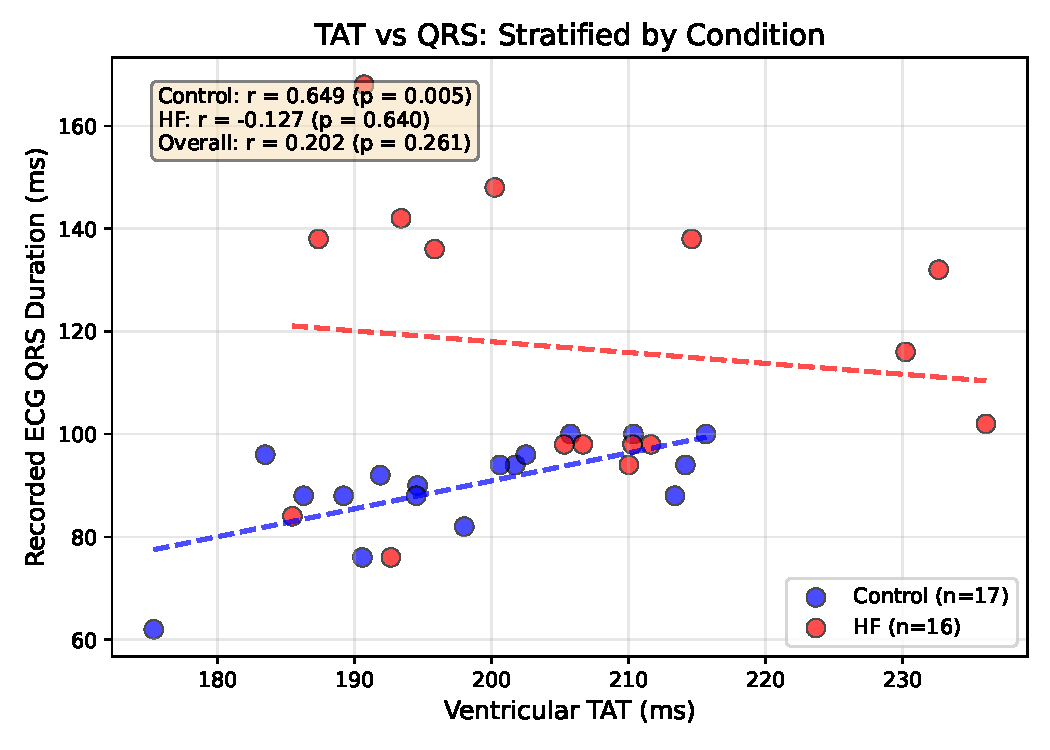
\includegraphics[width=\textwidth]{../pics/sp1_supp_tat_qrs_stratified.pdf}
    \caption{
        \textbf{Correlation between simulated ventricular total activation time
        (\TAT{V}) and recorded ECG QRS duration, stratified by condition.}
        In \Ctl{} hearts (blue, $n=17$), \TAT{V} showed a strong positive
        correlation with QRS duration (Pearson $r = 0.649$, $p = 0.005$),
        indicating that anatomical variability alone can predict conduction time
        in healthy myocardium when using uniform electrophysiological parameters.
        In \HF{} patients (red, $n=16$), no correlation was observed
        ($r = -0.127$, $p = 0.64$), reflecting that pathological conduction
        delays (fibrosis, scar, conduction blocks) are not captured by anatomy
        alone and would require patient-specific tissue property calibration.
    }
    \label{fig:s1-tat-qrs}
\end{figure}
